\newpage
\section{Power consumption measurements}
We ask you to measure the \textbf{power consumption} profile of the different
components of the embedded system, namely, the \textbf{MCU}, the \textbf{radio},
the \textbf{AFE} and the \textbf{total} consumption of the full system.
To measure the current consumed, you will insert
a \emph{shunt resistor} on the supply line of the device you
measure as in \autoref{fig:measure}. Please make sure you read carefully the last version
of the guide providing details on how to use the boards (see in the folder \texttt{Technical resources} on Moodle).

Practically, you can use the available jumpers as a way of inserting the
resistor. Dedicated jumpers are available on the MCU and the radio boards.
For the AFE, you must use the \textit{AFE\_SUP} selection header where you can
use the connections of the jumper for inserting the resistor.

The value for the shunt resistor is an important parameter of your measurement
setup: if this value is too low or too high, you will not get useful and
accurate measurements. You should be able to justify your choice.
You have access to a large set of resistors during the consultancy sessions.

Finally, we ask you to compare the power consumption of your system with the power that you will be able to harvest
in the future, thanks to the energy harvesting part of the circuit and the PV cells. (\textbf{Hint}: take a look at the data sheet and the characterization of the PV cell that we provided you in the folder \texttt{Technical resources} on Moodle). Does it fit ? Please provide a detailed explanation.

% \begin{figure}[h]
%     \centering
%     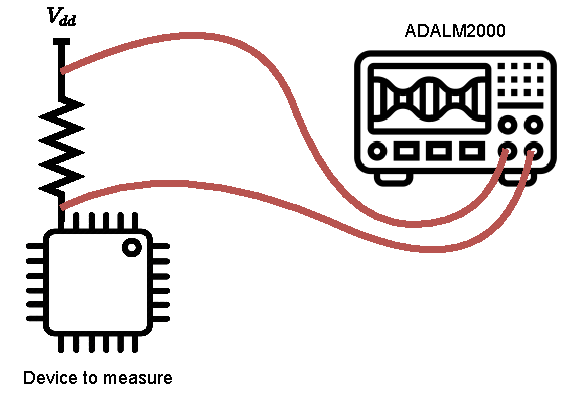
\includegraphics[width=0.35\textwidth]{figs/measure.pdf}
%     \caption{%
%         How to measure current consumption of a device. You can also use the
%         \textit{ADALM2000} to generate a power supply voltage of your choice.
%         Stay under the \SI{3.6}{V}, which is the maximum supply voltage of some
%         components in the system.
%     }
%     \label{fig:measure}
% \end{figure}

\begin{bclogo}[couleur = gray!20, arrondi = 0.2, logo=\bcinfo]{Differential probing}
        Contrary to the oscilloscopes of the Marconi lab, the
        \textit{ADALM2000} is a differential oscilloscope, meaning that there
        is no ground on the probe: both probe lines can be at any voltage.
        Therefore, you can use a single channel!
\end{bclogo}
\begin{bclogo}[couleur = gray!20, arrondi = 0.2, logo=\bcattention]{Measure real life conditions}
        Make sure to set up your device for a close to real life usage : Power
        it from an \textbf{external power supply} (as the PV cells would do)
        and not USB. In this mode, you must also make sure to deactivate the
        UART communication in the \texttt{config.h} file to avoid powering the
        ST-link in an undesired way.
\end{bclogo}
